% GNUPLOT: LaTeX picture with Postscript
\begingroup
  \makeatletter
  \providecommand\color[2][]{%
    \GenericError{(gnuplot) \space\space\space\@spaces}{%
      Package color not loaded in conjunction with
      terminal option `colourtext'%
    }{See the gnuplot documentation for explanation.%
    }{Either use 'blacktext' in gnuplot or load the package
      color.sty in LaTeX.}%
    \renewcommand\color[2][]{}%
  }%
  \providecommand\includegraphics[2][]{%
    \GenericError{(gnuplot) \space\space\space\@spaces}{%
      Package graphicx or graphics not loaded%
    }{See the gnuplot documentation for explanation.%
    }{The gnuplot epslatex terminal needs graphicx.sty or graphics.sty.}%
    \renewcommand\includegraphics[2][]{}%
  }%
  \providecommand\rotatebox[2]{#2}%
  \@ifundefined{ifGPcolor}{%
    \newif\ifGPcolor
    \GPcolorfalse
  }{}%
  \@ifundefined{ifGPblacktext}{%
    \newif\ifGPblacktext
    \GPblacktexttrue
  }{}%
  % define a \g@addto@macro without @ in the name:
  \let\gplgaddtomacro\g@addto@macro
  % define empty templates for all commands taking text:
  \gdef\gplbacktext{}%
  \gdef\gplfronttext{}%
  \makeatother
  \ifGPblacktext
    % no textcolor at all
    \def\colorrgb#1{}%
    \def\colorgray#1{}%
  \else
    % gray or color?
    \ifGPcolor
      \def\colorrgb#1{\color[rgb]{#1}}%
      \def\colorgray#1{\color[gray]{#1}}%
      \expandafter\def\csname LTw\endcsname{\color{white}}%
      \expandafter\def\csname LTb\endcsname{\color{black}}%
      \expandafter\def\csname LTa\endcsname{\color{black}}%
      \expandafter\def\csname LT0\endcsname{\color[rgb]{1,0,0}}%
      \expandafter\def\csname LT1\endcsname{\color[rgb]{0,1,0}}%
      \expandafter\def\csname LT2\endcsname{\color[rgb]{0,0,1}}%
      \expandafter\def\csname LT3\endcsname{\color[rgb]{1,0,1}}%
      \expandafter\def\csname LT4\endcsname{\color[rgb]{0,1,1}}%
      \expandafter\def\csname LT5\endcsname{\color[rgb]{1,1,0}}%
      \expandafter\def\csname LT6\endcsname{\color[rgb]{0,0,0}}%
      \expandafter\def\csname LT7\endcsname{\color[rgb]{1,0.3,0}}%
      \expandafter\def\csname LT8\endcsname{\color[rgb]{0.5,0.5,0.5}}%
    \else
      % gray
      \def\colorrgb#1{\color{black}}%
      \def\colorgray#1{\color[gray]{#1}}%
      \expandafter\def\csname LTw\endcsname{\color{white}}%
      \expandafter\def\csname LTb\endcsname{\color{black}}%
      \expandafter\def\csname LTa\endcsname{\color{black}}%
      \expandafter\def\csname LT0\endcsname{\color{black}}%
      \expandafter\def\csname LT1\endcsname{\color{black}}%
      \expandafter\def\csname LT2\endcsname{\color{black}}%
      \expandafter\def\csname LT3\endcsname{\color{black}}%
      \expandafter\def\csname LT4\endcsname{\color{black}}%
      \expandafter\def\csname LT5\endcsname{\color{black}}%
      \expandafter\def\csname LT6\endcsname{\color{black}}%
      \expandafter\def\csname LT7\endcsname{\color{black}}%
      \expandafter\def\csname LT8\endcsname{\color{black}}%
    \fi
  \fi
  \setlength{\unitlength}{0.0500bp}%
  \begin{picture}(15306.00,10204.00)%
    \gplgaddtomacro\gplbacktext{%
      \csname LTb\endcsname%
      \put(1474,704){\makebox(0,0)[r]{\strut{} 0}}%
      \put(1474,1730){\makebox(0,0)[r]{\strut{} 5e+10}}%
      \put(1474,2756){\makebox(0,0)[r]{\strut{} 1e+11}}%
      \put(1474,3782){\makebox(0,0)[r]{\strut{} 1.5e+11}}%
      \put(1474,4808){\makebox(0,0)[r]{\strut{} 2e+11}}%
      \put(1474,5835){\makebox(0,0)[r]{\strut{} 2.5e+11}}%
      \put(1474,6861){\makebox(0,0)[r]{\strut{} 3e+11}}%
      \put(1474,7887){\makebox(0,0)[r]{\strut{} 3.5e+11}}%
      \put(1474,8913){\makebox(0,0)[r]{\strut{} 4e+11}}%
      \put(1474,9939){\makebox(0,0)[r]{\strut{} 4.5e+11}}%
      \put(1606,484){\makebox(0,0){\strut{} 0.05}}%
      \put(3269,484){\makebox(0,0){\strut{} 0.1}}%
      \put(4932,484){\makebox(0,0){\strut{} 0.15}}%
      \put(6595,484){\makebox(0,0){\strut{} 0.2}}%
      \put(8258,484){\makebox(0,0){\strut{} 0.25}}%
      \put(9920,484){\makebox(0,0){\strut{} 0.3}}%
      \put(11583,484){\makebox(0,0){\strut{} 0.35}}%
      \put(13246,484){\makebox(0,0){\strut{} 0.4}}%
      \put(14909,484){\makebox(0,0){\strut{} 0.45}}%
      \put(176,5321){\rotatebox{-270}{\makebox(0,0){\strut{}$M$ [$M_\odot$]}}}%
      \put(8257,154){\makebox(0,0){\strut{}$1/R$ [1/kpc]}}%
      \put(9588,6245){\makebox(0,0)[l]{\strut{}\textbf{Masse der Galaxis}}}%
      \put(9588,6025){\makebox(0,0)[l]{\strut{}}}%
      \put(9588,5805){\makebox(0,0)[l]{\strut{}Fitgleichung: $M(R) = \frac{a}{R}$}}%
      \put(9588,5585){\makebox(0,0)[l]{\strut{}}}%
      \put(9588,5365){\makebox(0,0)[l]{\strut{}$a = 2{,}146\pm0{,}037 \cdot 10^{10}$}}%
    }%
    \gplgaddtomacro\gplfronttext{%
    }%
    \gplbacktext
    \put(0,0){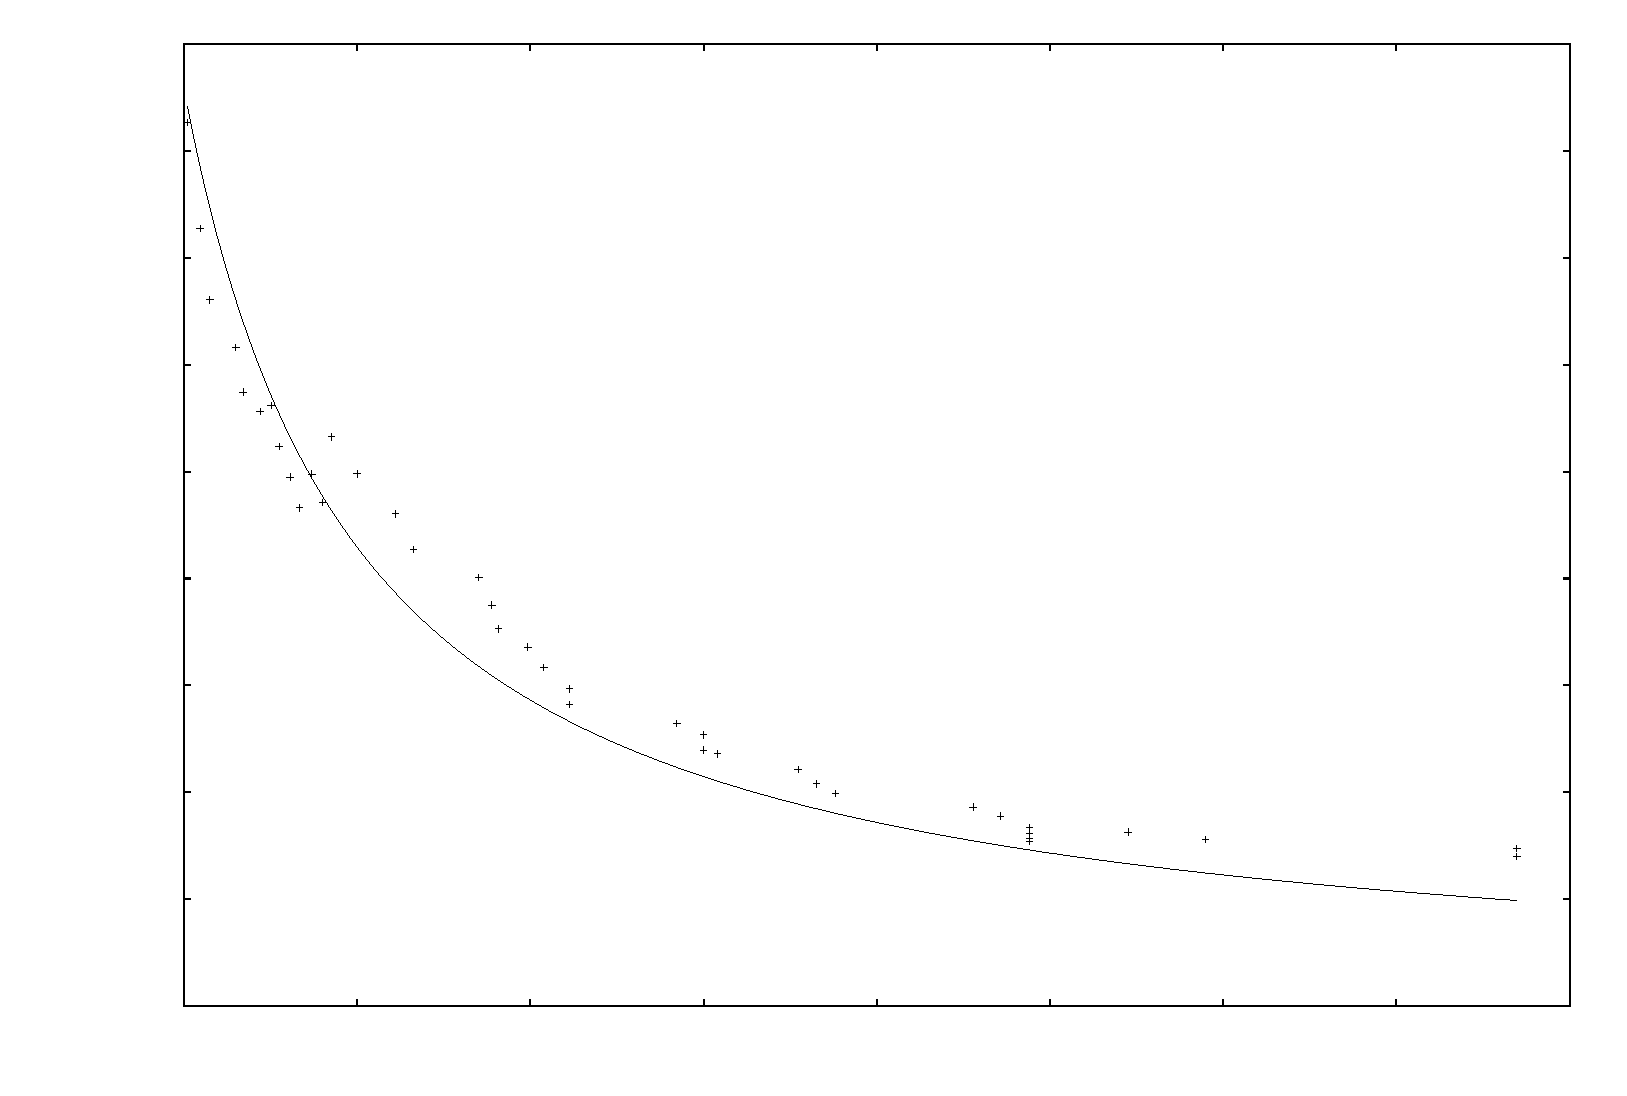
\includegraphics{plot-data-9}}%
    \gplfronttext
  \end{picture}%
\endgroup
